\section{Tarea}

\subsection{Objetivo}

\begin{itemize}
    \item Conocer el lenguaje de programación Scala.
    \item Resolver un ejercicio de programación propuesto con Scala.
    \item Responder las preguntas para reforzar el aprendizaje.
\end{itemize}


\subsection{Desarrollo}

\begin{enumerate}[label=\alph*.]
  \item Visite el sitio oficial de Scala u otros para estudiar el lenguaje de programación Scala.
  \item Estudie el problema recursivo propuesto.
  \item Resuelva el problema con el lenguaje de programación Scala (Recursivamente).
  \item Responda las tres preguntas formuladas.
\end{enumerate}


\subsection{Problema propuesto: Vuelto. Contando el vuelto o cambio.}

Escriba una función recursiva que cuente de cuántas maneras diferentes puede dar cambio para una determinada cantidad y de acuerdo a una lista de denominaciones de monedas.\\
Por ejemplo, hay 3 maneras de dar cambio si la cantidad=4 si tienes monedas con
denominación 1 y 2:
\begin{enumerate}[label={ }]
    \item 1+1+1+1,
    \item 1+1+2,
    \item 2+2.
\end{enumerate}

Realiza este ejercicio implementando la función countChange en Scala.
Esta función toma una cantidad a cambiar y una lista de denominaciones únicas para las
monedas.\\

Su definición es la siguiente:

\begin{verbatim}
    def countChange(money: Int, coins: List[Int]): Int
\end{verbatim}

Puedes usar las funciones isEmpty, head y tail en la lista de monedas enteras.



\section{Equipos, materiales y temas utilizados}

\begin{itemize}
    \item Subsistema de Windows para Linux (WSL) con Ubuntu (versión predeterminada instalada mediante Microsoft Store).
    \item Sistema operativo: Microsoft Windows [Versión 10.0.26100.6584]
    \item MiKTeX-pdfTeX 4.15 (MiKTeX 23.4) \LaTeX.
    \item Strawberry Perl (requerido por MiKTeX para la ejecución de scripts auxiliares en la compilación de ciertos paquetes).
    \item Helix 25.01.1 (e7ac2fcd)
    \item Visual Studio Code 1.104.0 x64
    \item Git version 2.41.0.windows.1
    \item Cuenta activa en GitHub para la gestión de repositorios remotos.
    \item Recursividad.
    \item Lenguaje de programación Scala.
    \item Compilador en línea programiz.com.
\end{itemize}



\section{URL de Repositorio Github}

\begin{itemize}
    \item URL del Repositorio GitHub para clonar o recuperar.
    \item \url{https://github.com/yhuayhuahi/Teo.git}
    \item URL para el laboratorio (\itemPracticeNumber) en el Repositorio GitHub.
    \item \url{https://github.com/yhuayhuahi/Teo/tree/main/laboratorios/lab\itemPracticeNumber}
\end{itemize}



\section{Desarrollo de las actividades}

\subsection {Actividades}

\subsubsection {Función propuesta}

Para resolver el problema propuesto se plantea la siguiente función recursiva en Scala:

\begin{lstlisting}[style=scala-custom, caption={Función countChange en Scala}]
    def countChange(money: Int, coins: List[Int]): Int = {
        if (money == 0) 1                // caso base hay 1 forma de dar cambio
        else if (money < 0) 0            // si la cantidad es negativa
        else if (coins.isEmpty) 0        // si no hay monedas disponibles no se puede dar cambio
        else {
            countChange(money - coins.head, coins) + countChange(money, coins.tail)
        }
    }
\end{lstlisting}

Se prueba el funcionamiento de la función en un compilador en línea, este es programiz.com:

\textbf{Función main:}

\begin{lstlisting}[style=scala-custom, caption={Función main para probar el funcionamiento de countChange}]
    @main def runCountChange(): Unit = {
        println("Ejemplo 01: 4 - [1,2]: " + countChange(4, List(1, 2)))    

        println("Ejemplo 02: 10 - [2, 5, 3, 6]: " + countChange(10, List(2, 5, 3, 6)))

        println("Ejemplo 03: 0 - [1, 2, 5]: " + countChange(0, List(1, 2, 5)))

        println("Ejemplo 04: 7 - [2, 4]: " + countChange(7, List(2, 4)))
    }
\end{lstlisting}

\begin{figure}[H]
    \centering
    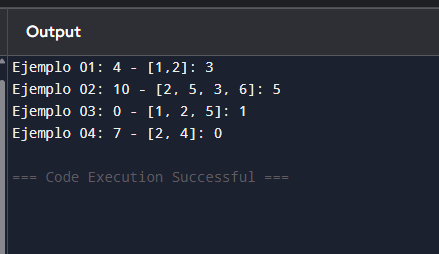
\includegraphics[width=0.8\textwidth]{img/prueba_ejecucion.png}
    \caption{Ejecución de la función countChange en compilador en línea programiz.com}
    \label{fig:compilador_en_linea}
\end{figure}

%\subsection {Commits realizados}

\subsection {Estructura del laboratorio}

A continuación se muestra la estructura de archivos y carpetas del laboratorio realizado:

\begin{figure}[H]
    \centering
    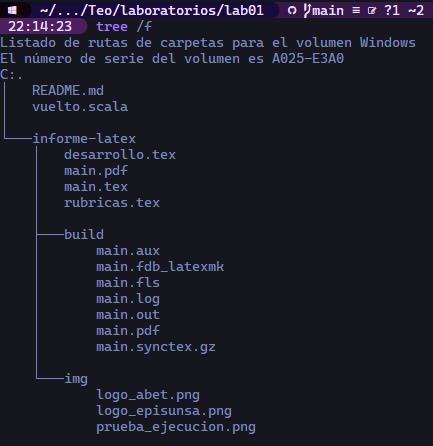
\includegraphics[width=0.6\textwidth]{img/estructura-lab01.png}
    \caption{Estructura de archivos y carpetas del laboratorio realizado}
    \label{fig:estructura_laboratorio}
\end{figure}

\section{Cuestionario}

\subsection{Explique el caso base implementado.}

En la función countChange, los casos base son los que permiten que la recursión se detenga. Son:

\begin{lstlisting}[style=scala-custom, caption={Casos base en la función countChange}]
    if (money == 0) 1
    else if (money < 0) 0
    else if (coins.isEmpty) 0
\end{lstlisting}

\begin{enumerate}[label={\alph*.}]
    \item \textbf{money == 0 → devuelve 1}
    Esto significa que si logramos llegar exactamente a 0, encontramos una forma válida de dar cambio (ya sea usando monedas o no).

    \item \textbf{money "<" 0 → devuelve 0}
    Si el valor del dinero se vuelve negativo, significa que usamos más monedas de las necesarias. Ese camino no genera solución válida.

    \item \textbf{coins.isEmpty → devuelve 0}
    Si ya no quedan monedas disponibles y todavía no llegamos a money==0, no podemos formar la cantidad. Entonces, no hay ninguna forma en ese camino.
\end{enumerate}


\subsection{¿Este problema se resuelve mejor en el modelo de programación funcional?}

Sí, este tipo de problema encaja muy bien en el modelo funcional por las siguientes razones:

\begin{enumerate}
    \item El problema se define de manera recursiva: “¿De cuántas formas puedo dar cambio con las monedas actuales?” se puede dividir en dos subproblemas más pequeños (usar o no usar una moneda). La recursión es un pilar de la programación funcional.
    \item En el enfoque funcional, las estructuras de datos (listas) son inmutables. Aquí no modificamos la lista de monedas ni el valor de money, simplemente pasamos nuevos valores a la recursión. Eso hace que el código sea más seguro y fácil de razonar.
    \item En vez de indicar cómo construir las combinaciones paso a paso (enfoque imperativo con bucles y mutaciones), describimos el problema con reglas simples. El compilador y la recursión se encargan del “cómo”.
\end{enumerate}


\subsection{¿Qué beneficios se podrían obtener para este problema utilizando memoización?}

El algoritmo recursivo puro tiene un gran inconveniente el cual es que repite muchos cálculos.

Se podría optimizar el rendimiento utilizando memoización, que es una técnica para almacenar los resultados de subproblemas ya resueltos y reutilizarlos cuando se vuelven a necesitar. Los beneficios serían:

\begin{enumerate}
    \item \textbf{Reducción de cálculos redundantes:} Almacenar los resultados de subproblemas evita que se recalculen múltiples veces, lo que mejora la eficiencia.
    \item \textbf{Mejora en el tiempo de ejecución:} Con menos cálculos que realizar, el tiempo de ejecución del algoritmo se reduce significativamente.
    \item \textbf{Facilidad para manejar problemas más grandes:} La memoización permite abordar problemas más complejos y de mayor tamaño sin un aumento exponencial en el tiempo de cálculo.
\end{enumerate}


